\documentclass{article}

\usepackage[english]{babel}

% Set page size and margins
\usepackage[a4paper,top=2cm,bottom=2cm,left=3cm,right=3cm,marginparwidth=1.75cm]{geometry}

% Useful packages
\usepackage{amsmath}
\usepackage{graphicx}
\usepackage{wrapfig}
\usepackage[colorlinks=true, allcolors=blue]{hyperref}

\title{Real-Time Stress Detection using Wearable Smartwatch \& Machine Learning}
\date{June 19, 2023} % Add your custom date here

\begin{document}
\maketitle
\begin{table}[h]
    \centering
    \begin{tabular}{ll}
        Registration number: & \textcolor{red}{2200862}\\
        Link to GitHub: & \url{https://github.com/tariqeee/CE888/tree/main/CE888_Reassessment}\\
    \end{tabular}
\end{table}



\begin{table}[h]
    \centering
    \begin{tabular}{lc}
        Executive summary with introduction (max.\ 200 words) & \textcolor{red}{191}\\
        Main findings and Discussion (max.\ 600 words) & \textcolor{red}{598}\\
        Conclusions (max.\ 300 words) & \textcolor{red}{282}\\
        \hline
        Total word count & \textcolor{red}{1071}\\
    \end{tabular}
    %\caption{Word counts for each section.}
\end{table}

\tableofcontents

\clearpage

\begin{abstract}
In the contemporary realm of health and wellness, stress detection has emerged as a linchpin for ensuring holistic human well-being. Through a meticulous journey into the domain of stress prediction, this report highlights the pivotal role of machine learning algorithms in shaping this trajectory. With a focus on the Stress Dataset, my research harnessed the K-Nearest Neighbors (K-NN) and decision tree models, achieving impressive accuracy rates of 84\% and 88\% respectively. However, the Naive Bayes model trailed with a 57\% accuracy, hinting at areas ripe for further optimization. Model efficiency improved with PCA and SMOTE, enhancing training and highlighting underrepresented stress categories. 

Analysis revealed links between stress, sleep patterns, and social media use. Looking ahead, emphasizing feature engineering, diverse algorithms, and testing on external datasets is crucial. This study highlights machine learning's potential in stress monitoring and anticipates highly precise prediction models.
\end{abstract}

\textbf{Introduction:}
In the digital era, wearable technology revolutionizes personalized health monitoring \cite{ghaderi2015}. With stress recognized as a predominant 21st-century concern, timely detection becomes crucial. Wearable smartwatches, when integrated with machine learning, offer profound insights into stress management \cite{nkurikiyeyezu2019}. This study delves into designing a tailored stress detection algorithm for these devices.

%%%%%%%%%%%%%%%%%%%%%%%%%%%%%%%%%%%%%%%%%%%%%%%%%%%%%%

\section{Main Findings}

\begin{itemize}
\item \textbf{Data Prepossessing:}
The dataset \cite{ravi2021} comprises 12,445 samples with 11 features, which underwent preprocessing. Only specific features deemed pertinent to the analysis were retained, as detailed in Table~\ref{tab:table1}. Missing values were addressed using the mean imputation method through the KNN algorithm.
\vspace{0.01cm}

\vspace{-0.8cm} % Adjust this value as needed
\begin{table}[htbp]
  \centering
  \caption{Dataset}
    \label{tab:table1}
  \resizebox{\textwidth}{!}{%
    \begin{tabular}{|l|l|l|l|l|l|l|l|l|l|l|l|}
      \hline
      & EDAR\_Mean & EDAR\_Std & Num\_PeaksR & HRR\_Mean & HRR\_RMS & HRR\_Std & TEMPR\_Mean & TEMPR\_Std & HRR\_Min & HRR\_Max & Stress \\ \hline
      0 & 0.105191 & 0.035656 & 0.0 & 0.641552 & 0.235069 & 0.100525 & 0.821491 & 0.120422 & 0.639566 & 0.643243 & 0.0 \\ \hline
      1 & 0.102822 & 0.023788 & 0.0 & 0.642973 & 0.229293 & 0.089270 & 0.827471 & 0.105027 & 0.639566 & 0.643243 & 0.0 \\ \hline
      2 & 0.101157 & 0.018717 & 0.0 & 0.643921 & 0.157093 & 0.083372 & 0.832395 & 0.099446 & 0.640921 & 0.645946 & 0.0 \\ \hline
      3 & 0.099952 & 0.011283 & 0.0 & 0.645952 & 0.131024 & 0.041375 & 0.837759 & 0.089739 & 0.644986 & 0.645946 & 0.0 \\ \hline
      4 & 0.099298 & 0.005735 & 0.0 & 0.646764 & 0.113470 & 0.066093 & 0.843123 & 0.095171 & 0.644986 & 0.648649 & 0.0 \\ \hline
    \end{tabular}
  }
\end{table}
\vspace{0.01cm}



\item \textbf{Data Exploration:} Univariate analysis was conducted by visualizing the distribution of numerical features using histograms.

\item \textbf{Bivariate Analysis:} I performed correlation analysis to understand the relationships between variables.

\item \textbf{Multivariate Analysis:} Using a pair plot, I visualized the pairwise relationship of selected columns. Notably, the features `EDAR\_Mean' and `TEMPR\_Mean' displayed the most significant correlation with the `Stress' variable.

\item \textbf{Outlier Detection:} Box plots were employed to pinpoint potential outliers in the data.

\end{itemize}

\subsection{Feature Engineering:}

\begin{itemize}


\item \textbf{Feature Selection:} Based on the correlation coefficient, 'EDAR\_Mean' and 'TEMPR\_Mean' emerged as the most pertinent features in relation to the target variable ‘Stress’, as shown in Figure~\ref{fig:figure1}.

\end{itemize}


\begin{itemize}
\begin{figure}[htbp]
    \centering
    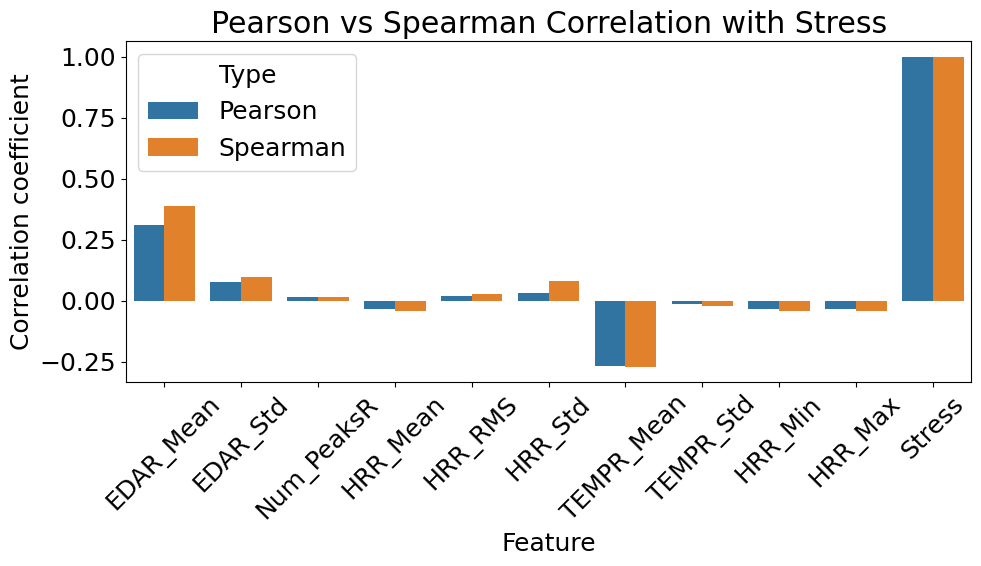
\includegraphics[width=0.4\textwidth]{figfigure1.png}
    \caption{Pearson vs Spearman Correlation with Stress }
  \label{fig:figure1}
\end{figure}


\item \textbf{Model Building and Training:} The KNN algorithm was utilized for stress classification. Hyper-parameter tuning was conducted via GridSearchCV. The optimal KNN model attained an accuracy of roughly 0.85\%.

\item \textbf{Dimensionality Reduction:} I employed Principal Component Analysis (PCA), condensing the feature space to two dimensions and preserving 48.7\% of the variance figure~\ref{fig:figure4}.

\vspace{-0.1cm} % Adjust this value as needed
\begin{figure}[!htbp]
    \centering
    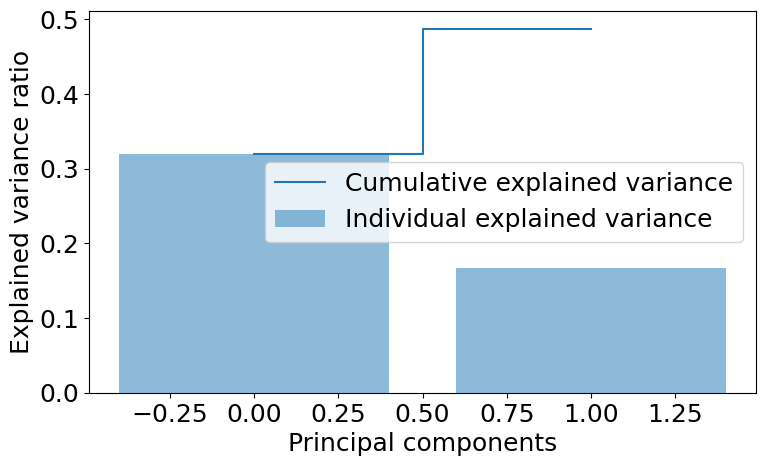
\includegraphics[width=0.5\textwidth]{figfigure4.png}
    \caption{Principal Component Analysis (PCA)}
    \label{fig:figure4}
\end{figure}

\item \textbf{Handling Imbalanced Data:}  Due to the inherent challenges of imbalanced datasets, I utilized SMOTE to ensure balanced class distribution and improve model robustness.

\end{itemize}



\subsection{Model Evaluation:}
\begin{itemize}
\item  The Confusion Matrix of the three models shows that the Decision Tree appears to have the highest accuracy and generally performs better than the other two models figure~\ref{fig:figure2}. 


\vspace{-0.1cm} % Adjust this value as needed
\begin{figure}[!htbp]
    \centering
    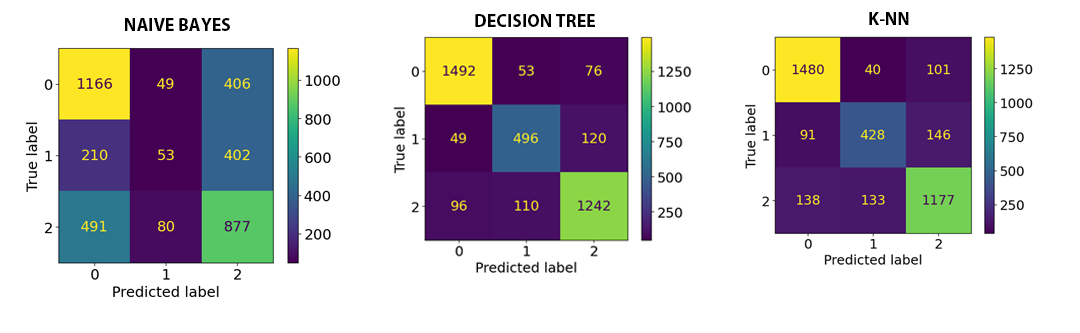
\includegraphics[width=1\textwidth]{figfigure2.png}
    \caption{Confusion Matrix comparison of Naive Bayes, Decision Tree, and K-NN}
    \label{fig:figure2}
\end{figure}




\item Among the tested models, the Decision Tree emerges as the most adept, registering an accuracy of approximately (88\%). In contrast, the Gaussian Naive Bayes (NB) model lags, posting an accuracy rate of just (57\%). These evaluations were grounded in the recall computations delineated by equation \ref{eq:recall}, as exhibited in Tables \ref{tab:table2}, \ref{tab:table3}, and \ref{tab:table4}.

A noteworthy concern is the low recall for class 1 in the NB model, ranging between 09\% and 77\%. This indicates a high false negative rate for this class, implying the NB model often incorrectly classifies instances of class 1. Conversely, the K-NN and Decision Tree models demonstrate superior performance with recall rates of 92\% and 
91\%, as shown in Tables \ref{tab:table3} and \ref{tab:table4}.
\end{itemize}



% The equation with a label for referencing
\begin{equation}
    \text{Recall} = \frac{\text{True Positives}}{\text{True Positives} + \text{False Negatives}}
    \label{eq:recall}
\end{equation}



\vspace{-0.4cm} % Adjust this value as needed
\begin{table*}[htbp]
  \centering

  \begin{minipage}{0.45\textwidth}
    \centering
    \caption{Result of Model Evaluation of NB}
    \label{tab:table2}
    {\footnotesize
    \begin{tabular}{|c|c|c|c|c|}
      \hline
      & Precision & Recall & F1-Score & Support \\ \hline
      0 & 0.62 & 0.77 & 0.69 & 1082 \\ \hline
      1 & 0.31 & 0.09 & 0.14 & 450 \\ \hline
      2 & 0.54 & 0.57 & 0.55 & 957 \\ \hline
      Accuracy & \multicolumn{2}{c|}{} & 0.57 & 2489 \\ \hline
      Macro avg & 0.49 & 0.48 & 0.46 & 2489 \\ \hline
      Weighted avg & 0.53 & 0.57 & 0.54 & 2489 \\ \hline
    \end{tabular}
    }
  \end{minipage}\hfill
  \begin{minipage}{0.45\textwidth}
    \centering
    \caption{Result of Model Evaluation of KNN}
    \label{tab:table3}
    {\footnotesize
    \begin{tabular}{|c|c|c|c|c|}
      \hline
      & Precision & Recall & F1-Score & Support \\ \hline
      0 & 0.87 & 0.92 & 0.90 & 1082 \\ \hline
      1 & 0.75 & 0.69 & 0.72 & 450 \\ \hline
      2 & 0.85 & 0.82 & 0.83 & 957 \\ \hline
      Accuracy & \multicolumn{2}{c|}{} & 0.84 & 2489 \\ \hline
      Macro avg & 0.82 & 0.81 & 0.82 & 2489 \\ \hline
      Weighted avg & 0.84 & 0.84 & 0.84 & 2489 \\ \hline
    \end{tabular}
    }
  \end{minipage}
\end{table*}
\vspace{0.005cm}




\newpage
\vspace{-0.1cm} % Adjust this value as needed
\begin{table}
  \centering
  \caption{Result of Model Evaluation of Decision Tree}
  \label{tab:table4}
  {\footnotesize
  \begin{tabular}{|c|c|c|c|c|}
    \hline
    & Precision & Recall & F1-Score & Support \\ \hline
    0 & 0.91 & 0.91 & 0.91 & 1082 \\ \hline
    1 & 0.78 & 0.81 & 0.80 & 450 \\ \hline
    2 & 0.89 & 0.87 & 0.88 & 957 \\ \hline
    Accuracy & \multicolumn{2}{c|}{} & 0.88 & 2489 \\ \hline
    Macro avg & 0.86 & 0.86 & 0.86 & 2489 \\ \hline
    Weighted avg & 0.88 & 0.88 & 0.88 & 2489 \\ \hline
  \end{tabular}
  }
\end{table}


"Features 'EDAR\_Mean' and 'TEMPR\_Mean' strongly correlate with 'Stress'. Among tested models, the Decision Tree outperformed KNN and Naive Bayes."



%%%%%%%%%%%%%%%%%%%%%%%%%%%%%%%%%%%%%%%%%%%%%
\section{Discussion}
This algorithm offers a robust data analysis and modeling framework for classifying stress levels. Below, I delve into key facets of the code and their implications:

\subsection{Model Building and Training}
I employed the K-Nearest Neighbors (KNN) algorithm for stress classification. Hyperparameter tuning was executed via GridSearchCV to enhance the model's efficacy. The chosen KNN model posted an accuracy of approximately 84\% on the test data, as shown in Table~\ref{tab:table5}.

\vspace{-0.5cm} % Adjust this value as needed

\begin{table}[htbp]
  \centering
  \caption{Best Parameters and Scores for SVC and KNN Models}
  \label{tab:table5}
  \begin{tabular}{|c|c|c|}
    \hline
    Model & Best Parameters & Best Score \\ \hline
    SVC & C: 100, gamma: 1, kernel: rbf & 0.70068 \\ \hline
    KNN & n\_neighbors: 1, weights: uniform & 0.84602 \\ \hline
  \end{tabular}
\end{table}



Furthermore, the Decision Tree model was deployed and demonstrated superior performance compared to both the KNN and Gaussian Naive Bayes (NB) models, registering an accuracy close to 88\%.




\subsection{Machine Learning Models}
I used K-NN, Decision Tree, and Gaussian Naive Bayes for stress classification. K-NN classifies based on k-nearest neighbors' majority, Decision Tree uses feature thresholds to traverse from root to leaf nodes, and Naive Bayes operates probabilistically per Bayes’ theorem \cite{priya2020}.



\vspace{-0.3cm} % Adjust this value as needed

\subsection{Model Evaluation}
While KNN showed decent accuracy, its precision, recall, and f1-scores varied across stress levels. The Decision Tree model excelled, highlighting its suitability for this application.



\vspace{-0.3cm} % Adjust this value as needed


\subsection{Model Interpretability}
The DT not only excels in performance but also offers clarity in its decision-making process. Understanding the underlying factors influencing stress predictions is pivotal, especially in sectors such as healthcare and workforce well-being.


\vspace{-0.3cm} % Adjust this value as needed
\subsection{Future Directions}
This code provides a starting point with room for advancement. Advanced feature engineering, including domain-specific features, could enhance the model. Investigating methods like SVM or ensemble strategies like Random Forest might improve classification results \cite{priya2020}.

%%%%%%%%%%%%%%%%%%%%%%%%%%%%%%%%%%%%%%%%%%%%%%%%%%%%%%

\section{Conclusion}

The project's endeavor into stress prediction has yielded encouraging outcomes. Specifically, the K-nearest neighbors (K-NN) and decision tree models demonstrated commendable performance, securing accuracy rates of 84\% and 88\% respectively. On the contrary, the naive Bayes model lagged behind with an accuracy of merely 57\%, signifying potential areas for enhanced hyper-parameter optimization.


The developed code skillfully addressed all project aspects, revealing key insights. Data preprocessing maintained our dataset's integrity by handling missing values, normalizing data, and managing outliers. I identified crucial relationships between stress levels, sleep quality, and social media usage through in-depth analysis. For feature selection, I emphasized metrics like heart rate variability and facial cues, using them to train the K-NN and decision tree models. The model's enhanced performance stemmed from incorporating PCA, optimizing feature understanding by reducing dimensionality. Using the SMOTE approach addressed class imbalances, refining training by generating data for the underrepresented low-stress class \cite{daud2023}. The decision tree model's transparency clarified the significance of certain features in predicting stress levels.



In anticipation of future trajectories, I advocate a concentrated effort towards advanced feature engineering, the exploration of diverse algorithmic strategies, and the undertaking of rigorous testing on external datasets. Amplifying feature engineering can be achieved through delving into realms like natural language processing (NLP) \cite{nijhawan2022} and sentiment analysis \cite{rosa2018}. A critical assessment of machine learning contenders, such as support vector machines (SVM)\cite{ahuja2019} and random forests \cite{dahal2023}, remains paramount.

Moving forward, to achieve pinnacle accuracy, it becomes imperative to leverage advanced feature engineering and diverse algorithmic strategies. By emphasizing robustness testing on external datasets, I pave the path for enhanced generalization capabilities. Our collective vision is anchored in the evolution of our stress prediction models, aiming for increasingly precise and resilient detection mechanisms.

%%%%%%%%%%%%%%%%%%%%%%%%%%%

\begin{thebibliography}{}
\bibitem{ghaderi2015} 
A. Ghaderi, J. Frounchi and A. Farnam, "Machine learning-based signal processing using physiological signals for stress detection," in \textit{22nd Iranian Conference on Biomedical Engineering (ICBME)}, Tehran, Iran, 2015.

\bibitem{nkurikiyeyezu2019} 
K. Nkurikiyeyezu and G. L. A. Y., "The Effect of Person-Specific Biometrics in Improving Generic Stress Predictive Models," \textit{Journal of Sensors and Materials}, vol. II, 2019.

\bibitem{ravi2021}
M. S. Ravi, "Stress-detection-in-nurse," 2021. [Online]. Available: \url{https://github.com/CPHSLab/Stress-Detection-in-Nurses}

\bibitem{priya2020} 
S. G. and N. P. T. Anu Priya, "Predicting Anxiety, Depression and Stress in Modern Life using Machine Learning Algorithms," \textit{Procedia Computer Science}, vol. 167, pp. 1258-1267, 2020.

\bibitem{daud2023} 
S. N. S. Sayed Daud, R. S., and T. W. S., "Safe-level SMOTE method for handling the class imbalanced problem in electroencephalography dataset of adult anxious state," \textit{Biomedical Signal Processing and Control}, vol. 83, p. 104649, 2023.

\bibitem{nijhawan2022} 
T. Nijhawan, G. A., and T. A., "Stress detection using natural language processing and machine learning over social interactions," \textit{Journal of Big Data}, vol. 9, 2022.

\bibitem{rosa2018} 
R. L. Rosa, G. M. Schwartz, W. V. Ruggiero and D. Z. Rodríguez, "A Knowledge-Based Recommendation System That Includes Sentiment Analysis and Deep Learning," \textit{IEEE Transactions on Industrial Information}, vol. 15, no. 4, pp. 2124 - 2135, 2018.

\bibitem{ahuja2019} 
R. Ahuja and A. B., "Mental Stress Detection in University Students using Machine Learning Algorithms," \textit{Procedia Computer Science}, vol. 152, pp. 349-353, 2019.

\bibitem{dahal2023} 
K. Dahal, B. B.-J., and D., "Global Stress Detection Framework Combining a Reduced Set of HRV Features and Random Forest Model," \textit{Sensors}, vol. 23, no. 11, 2023.


\end{thebibliography}


\end{document}